% Source: tex/chapters/ch06/06_ソフトウェアエンジニアリング運用提供.tex
\subsubsection{配備・リリース工学}

配備とは、指定された版のソフトウェアを、特定の環境へインストールすることである。リリースとは、機能または機能集合を、顧客や利用者が実際に使える状態にすることである。配備とリリースは似ているが、同じではない。配備は技術的な配置であり、リリースは利用可能にする判断である。

\par\smallskip\noindent\refstepcounter{table}\label{tab:ch06-06}\textbf{表 \thetable: 第06章 ソフトウェアエンジニアリング運用 表06}\par\smallskip
\begin{longtable}{L{35mm}L{115mm}}
\toprule
概念 & 説明 \\
\midrule
配備 & コード、設定、データベース、サーバ、コンテナなどを対象環境へ置き、動作可能にする技術的活動である。 \\
リリース & 配備済みの機能を、すべての利用者または一部の利用者に使えるようにする活動である。ビジネス判断を含む。 \\
\bottomrule
\end{longtable}

従来は、開発チームが完成物を運用チームに引き渡し、運用チームが手作業で配備することが多かった。この方法は時間がかかり、品質面でもリスクがある。DevOpsでは、コードの包装、設定ファイル生成、サーバ再起動、サーバとデータベースの設定、ソフトウェアのインストール、アプリケーション起動、スモークテストを自動化する。

リリース戦略には、環境に基づく戦略とアプリケーションに基づく戦略がある。環境に基づく戦略では、新版を事前本番環境や別環境へ配備してから切り替える。アプリケーションに基づく戦略では、機能トグルのような設定により、コード中の特定機能を有効化または無効化する。

カナリアリリースは、変更を一部の範囲にだけ短期間配備し、その結果を評価してから全面配備を判断する方法である。新しいソフトウェアが異常を示した場合、自動的にロールバックできる構成も重要である。

\begin{figure}[htbp]
\centering
\IfFileExists{assets/fig-ch06-07.png}{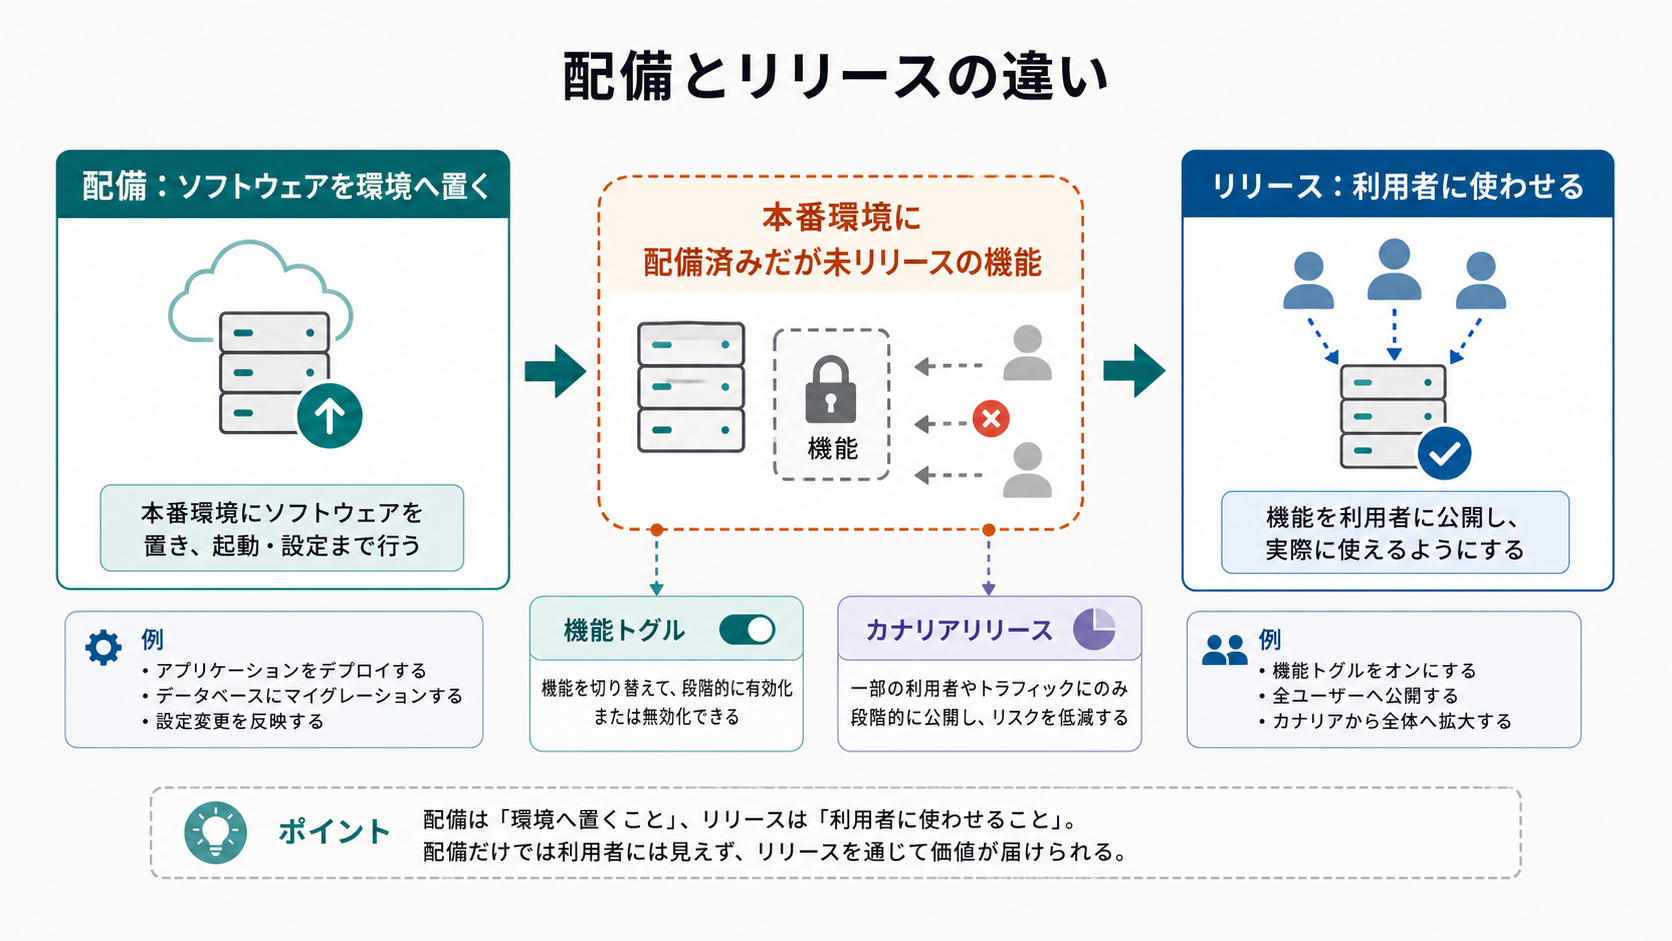
\includegraphics[width=0.96\linewidth]{assets/fig-ch06-07.png}}{\fbox{\parbox[c][48mm][c]{0.9\linewidth}{\centering 画像生成待ち\\配備とリリースの違い}}}
\caption{配備とリリースの違い}
\label{fig:ch06-07}
\end{figure}
